\documentclass{book}

\usepackage{graphicx}
\usepackage{psfrag}
\usepackage{makeidx}  % allows for indexgeneration
\usepackage{multirow}
\usepackage{psfrag}
\usepackage{caption}
\usepackage{amsmath}
\usepackage{setspace}
\usepackage{listings}

\begin{document}

\begin{titlepage}
\begin{center}

\begin{spacing}{2.5}
\textbf{\huge The 1chipML library}\\[0.5cm]

\begin{figure}[h]
\centering
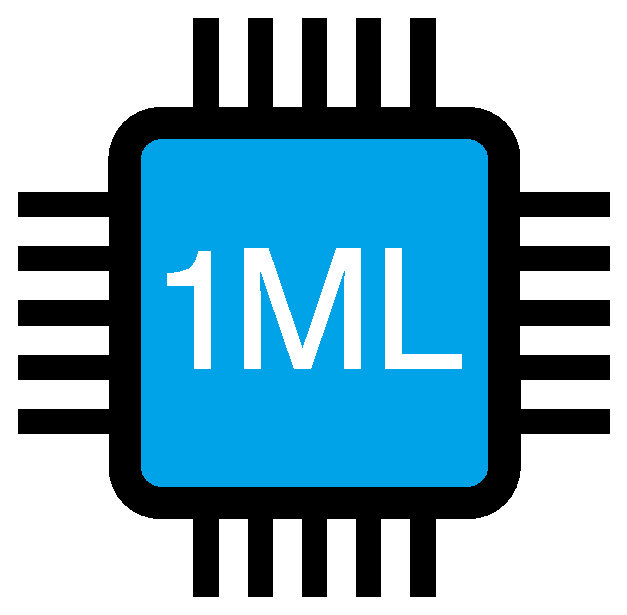
\includegraphics[width=0.3\textwidth]{1chipML_logo.eps}
\end{figure}

\vspace*{\fill}
\textit{Manual written and maintained by}
\end{spacing}

\begin{spacing}{1.15}
\textbf{\large Jean Michel Sellier$^*$}
\vspace*{\fill}
\end{spacing}

\begin{spacing}{1.15}
\textit{\large in collaboration with}

\textbf{Qinan Qi, Hardik Dalal,\\Yimin Nie, Salman Memon.}

\vspace*{\fill}

\textnormal{\large $^*$Global Artificial Intelligence Accelerator,\\ Ericsson, Montr\'{e}al,\\Qu\'{e}bec, Canada\\ \bigskip manual version 20220510}

\end{spacing}
\end{center}
\end{titlepage}

\tableofcontents

\chapter{What is 1chipML?}

\section{Introduction}

The Internet of Things (IoT) and Edge Computing (EC) are, nowadays, topics of high interest since
it is becoming clear that important advantages could emerge from this new sort of    technologies.
What kind of hardware will be in use in this context is still work in progress         since many
different directions are currently being explored.

In more details, one can consider the IoT as an ensemble        of computing objects with sensors,
embedded software, etc., which can connect and exchange data with other devices over the Internet
(or, equivalently, other communication networks). A continuously growing number of    IoT devices
are already being created for connected vehicles, home automation, wearable technology, and   all
sort of appliances with remote monitoring capabilities.         For instance, in industry, we are
witnessing the creation of a growing number of IoT devices       to acquire and analyze data from
connected equipment, operational technology, locations, and people.      Combined with monitoring
devices, this new technological paradigm is helping to regulate and monitor industrial    systems.
The same approach can be applied for automated record updates    of asset placement in industrial
storage units. Another important example of IoT is represented by the  Internet of Medical Things
(IoMT) which can be considered as an application of the IoT for medical and        health related
purposes. This novel technology can help in the creation         of a digitized healthcare system,
connecting available medical resources and healthcare services.

Edge computing is a growing and relevant approach as well, but very different than the IoT.    In
practice, the aim of edge computing is to move the computation away from data centers towards the
edge of the network, exploiting smart objects, mobile phones,      or network gateways to perform
tasks and provide services on behalf of the cloud.      Therefore, it also can be considered as a
distributed computing  paradigm that brings computation and data storage closer to the sources of
data. In other words, one can consider the EC as any type of computer   program which can deliver
low latency nearer to the requests. Thus, this new computing approach is expected     to speed up
response times and save bandwidth since it is possible to provide content caching,        service
delivery, persistent data storage,      and IoT management resulting in better response times and
transfer rates.

Obviously, the sort of hardware needed to implement these two approaches cannot solely    rely on
classical computing devices such as servers, Beowulf clusters, etc.      since they require those
devices to be fast, low power demanding and in small packages. One technology approach that seems
to be currently emerging is based on the use of microcontrollers (MCUs). While this seems to be a
promising direction, it obviously comes with new challenges which needs to be addressed.    Among
these open problems, one that seems to be relevant nowadays   is the lack of a available software
infrastructures for the fast development of such technologies. 1chipML is a library which purpose
is to bridge this gap.

\section{1chipML in a nutshell}

In order to make a technology take off,        it is important to have a fast and reliable way to
develop (and evolve) it.      Without such infrastructure and tools, it is hard to imagine how to
develop something that can have a real impact on society.       In fact, the availability of such
infrastructure can become the very reason for the success (or failure) of an invention, no matter
what the field is. Obviously, this is valid for the fields of IoT and EC too.      At the time of
writing this manual, one quickly realizes (unfortunately) that such development         tools are
practically unavailable, especially if the goal is to run relatively sophisticated  algorithms on
MCUs such as number crunching and machine learning (ML) methods.        Of course, there are some
available libraries but they are either proprietary (or incomplete),  which is known to slow down
the development of technology      (a great example is provided by the GNU/Linux operating system
which has, eventually, allowed the development of the Android operating system).      The goal of
1chipML is to bridge this gap so that IoT and EC can become quickly mainstream.

The target of the 1chipML team of volunteers is to develop and maintain a library       which can
provide relevant computational capabilities on MCUs related to number crunching and ML.       For
example, one could need to run the Gauss elimination method to solve a relatively small system of
linear equations. The only option for now is to develop everything from scratch which can be time
consuming and error prone. With the 1chipML library, this problem is solved.  One simply needs to
download it and use it right away. A practical example is reported in a section below.

At the time of writing this manual,  there  are  relevant  main families of MCUs available on the
market such as the ones produced by ARM and AVR.  While,  in the past, these MCUs used to be very
limited (with very limited amount of memory and computational power), nowadays they have features
which allow to run relatively complex algorithms on such devices which used     to be practically
impossible previously. This is one of the reasons why 1chipML has been created.


\section{Development paradigms}

How to use 1chipML? There are essentially two ways:
\begin{itemize}
 \item It is possible to include the whole library into a code so that all methods implemented are available at once.
 \item It is possible to include only the algorithm that is needed. In this case, only the relevant methods are included.
\end{itemize}

A first practical example is discussed below.

\section{A first example}

\lstset{language=C}

The Gauss elimination method, also known as row reduction method, is an algorithm  to       solve
systems of linear equations. This method consists  of  a  sequence of operations performed on the
matrix of coefficients corresponding to the system at hand.         To perform the computation, a
sequence of elementary row operations which modifies the matrix until  the lower left-hand corner
of the matrix is filled with zeros, as much as possible.

This method is available in the 1chipML library and it is very simple to use it.    The user does
not  need  to  implement anything related to number crunching beyond the definition of the linear
system itself.




\begin{lstlisting}
#include<stdio.h>
#include<stdlib.h>
#include<math.h>

#include "../src/1chipml.h"

int main(void){
 /* Variables and pointers declarations */
 int i;
 int N;
 gauss_real A[2][2];
 gauss_real B[2];
 gauss_real *sol; /* pointer towards the solution */

 /* The following parameters define a system of 2 linear equations A*X=B */
 N=2;
 A[0][0]=+1.; A[0][1]=+1.;
 A[1][0]=+1.; A[1][1]=-1.;
 B[0]=0.;
 B[1]=1.;

 /* Apply gauss elimination method to solve the system */
 sol=gauss_elimination(N,A,B);

 /* Print solution on screen */
 for(i=0;i<N;i++) printf("sol[%d] = %0.3f\n",i,sol[i]);
 return(0);
}
\end{lstlisting}

\chapter{Numerical crunching}

This chapter introudces and discusses the various numerical methods that are already implemented in the current version of the library.
The Reader should bear in mind that this is still work in progress at the moment.

\section{Random number generators}

The generation of random numbers is a process used to create a sequence of numbers which cannot be reasonably predicted.
Two main methods are used to generate random numbers. In the first approach, one measures some physical phenomenon that
is expected to be random and then compensates for possible biases in the measurement process. For instance, sources of
randomness include measuring atmospheric noise, thermal noise, and other external electromagnetic and quantum phenomena.
In the second approach, one uses computational algorithms that can produce long sequences of apparently random results,
which are in fact completely determined by a shorter initial value, known as a seed value or key. This type of random
number generator is often called a pseudorandom number generator and it is the method used in the 1chipML library.

While a pseudorandom number generator based solely on deterministic logic can never be regarded as a true random number
source in the purest sense of the word, in practice they are generally sufficient even for demanding security-critical
applications. In fact, carefully designed and implemented pseudorandom number generators can be certified for security-critical
cryptographic purposes. Many computational methods exist for pseudorandom number generation. In the following we present two of these pseudorandom number generators.

\subsection{The linear congruential generator}

This method is implemented in the file "src/linear\_congruential\_random\_generator.c" of the library.

A linear congruential generator is an algorithm that yields a sequence of pseudo-randomized numbers computed
with a discontinuous piecewise linear equation. This method represents one of the oldest and best-known pseudorandom
number generator algorithms. The theory behind them is relatively easy and, consequently, allow a fast and easy implemention.

The main idea behind this generator is to use the following recursive relation:
$$
 X_{(n+1)} = (a X_n + c) \pmod m,
$$
where $X_{(n+1)}$ and $X_n$ are values in the sequence of pseudorandom numbers, and $X_0$ is called the seed or start value of the sequence.
The constants $a$, $c$ and $m$ are known as the multiplier, the increment and the modulus respectively with $m>0$, $0<a<m$ and $0 \le c<m$. In our particular
implementation of this method, the values for these constants are $a=1027$, $c=0$ and $m=1048576$. The initial seed $X_0$ is set to $38467$ by default. The user
can modify it by using the following command:
\begin{lstlisting}
 ISEED = some_value;
\end{lstlisting}

For clarity, an extract of the file "tests/test\_linear\_congruential\_random\_generator.c" is reported below:
\begin{lstlisting}
 /* Variables and pointers declarations */
 int i,n=100;

 printf("linear congruential random generator\n");
 for(i=0;i<n;i++) printf("%1.3f ",linear_congruential_random_generator());
\end{lstlisting}

\subsection{The Mersenne twister}

Work in progress. This method is not implemented in the library yet.


\section{Systems of linear equations}

A system of linear equations is simply a collection of one or more linear equations involving the same variables.
The theory of linear systems is the basis and a fundamental part of linear algebra, a subject which is used in
most parts of modern mathematics. Computational algorithms for finding the solutions are an important part of
numerical linear algebra, and play a prominent role in engineering, physics, chemistry, computer science, and economics.
In the following we present the methods implemented in the library.

\subsection{The Gaussian elimination method}

This method is implemented in the file "src/gauss\_elimination.c" of the library.

The Gaussian elimination method, also known as row reduction, is an algorithm used to
solve systems of linear equations. It consists of a sequence of operations, i.e. row reductions, performed
on the corresponding matrix of coefficients. This method can also be used to compute
the rank of a matrix, the determinant of a square matrix, and the inverse of an invertible matrix. 

To perform row reduction on a matrix, one uses a sequence of elementary row operations to modify
the matrix. There are three types of elementary row operations, i.e. {\sl{1)}} swapping two rows,
{\sl{2)}} multiplying a row by a nonzero number, and {\sl{3)}} adding a multiple of one row to another row.
Using these operations, a matrix can always be transformed into an upper triangular matrix, and in fact one
that is in row echelon form. Once all of the leading coefficients are equal to 1, and every column containing
a leading coefficient has zeros elsewhere, the matrix is said to be in reduced row echelon form.
This final form is unique, i.e. it is independent of the sequence of row operations used, and it is this form
that is utilized to find the solutions of the system at hand.

To better understand how to use this method implemented in the library, an extract of the file "tests/test\_gauss\_elimination.c" is reported below:
\begin{lstlisting}
 /* Variables and pointers declarations */
 int i;
 int N;
 gauss_real A[2][2];
 gauss_real B[2];
 gauss_real *sol; /* pointer towards the solution */

 /* The following parameters define a system of 2 linear equations A*X=B */
 N=2;
 A[0][0]=+1.; A[0][1]=+1.;
 A[1][0]=+1.; A[1][1]=-1.;
 B[0]=0.;
 B[1]=1.;

 /* Apply gauss elimination method to solve the system */
 sol=gauss_elimination(N,A,B);

 /* Print solution on screen */
 for(i=0;i<N;i++) printf("sol[%d] = %0.3f\n",i,sol[i]);
 return(0);
\end{lstlisting}

\subsection{The LU decomposition method}

Work in progress. This method is not implemented in the library yet.

\section{Interpolation and extrapolation}

Work in progress.

\subsection{Polynomial-based approach}

Work in progress.

\subsection{Spline-based approach}

Work in progress.

\section{Optimization problems}

Work in progress.

\subsection{The gradient descent method}

Work in progress.

\subsection{The genetic approach}

Work in progress.

\section{Numerical derivation and integration}

Work in progress.

\subsection{First and second order finite differences approach}

Work in progress.

\subsection{The Monte Carlo approach}

The file "src/mc\_integration.c " describes the function of doing integration with Monte Carlo approach.
One can examine the expected value of an integral using the Monte Carlo approach. Traditionally, the
expected value of a function $g(x)$ can be calculated by first multiplying by its probability density function,
$f(x)$, and taking the integral over the desired region:
$$
 E [ g(x) ] = \int_a^b g(x) f(x) dx
$$
Alternatively, we can use a Monte Carlo approximation for the expected value by repeatedly
sampling a uniform distribution between the limits of integration.
$$
 E [ g(x) ] = \frac{1}{n} \sum_{i=1}^n f(x_i)
$$
where $x_i \in [a, b]$. As noted, $x_i$  is a value that is sampled from a uniform distribution
between the limits $a$ and $b$ for each unique $n = 1,2,3,$ etc. This approach samples the $f(x)$
function and uses the law of large numbers to find a converged expected value.
As an aside, the multiplicative factor of $1/n$ is sometimes given as $1/(n-1)$ because there are
truly $n-1$ degrees of freedom with $n$-samples, but when $n$ is large enough the difference between
$1/n$ and $1/(n-1)$ is negligible.

Given the form of the estimator for the expected value, extending to the estimate of the integral is simple.
The expected value formula is multiplied by the range of the integration limits, as shown below.
$$
 F = (b-a) \frac{1}{n} \sum_{i=1}^n f(x_i)
$$
where $x_i \in [a, b]$.

The file "src/mc\_std.c" describes how to calculate variance using the Monte Carlo approach. The variance of
the Monte Carlo integration scheme follows a traditional process of calculating variance around some random variable.
By continuing with the notation of taking the integral of a function $g(x)$, and the expected value of the integral being $E[g(x)]$,
the relationship for standard deviation can be given as:
$$
 \sigma_n = V \sqrt{\frac{E[g(x)^2] - E[g(x)]^2}{n-1}}.
$$
Here the additional $V$ term represents the total volume of the integration limits. If we were to evaluate a one-dimensional
integral between the limits of $a$ to $b$ then the equation could be written as:
$$
 \sigma_n = (b-a) \sqrt{\frac{E[g(x)^2] - E[g(x)]^2}{n-1}}.
$$
Using this format, we can easily calculate standard deviation or variance (standard deviation$^2$ = variance) along with the integration estimate.

The file "src/mc\_stratified\_sampling.c" is concerned with stratified sampling which is an approach to variance reduction
by which the integration volume is divided into subdomains that are each evaluated separately. The estimates from each
subdomain are then combined with a weight depending on their subdomain integration volume. Stratified sampling has the
benefit of always reducing the sample variance, without any prior knowledge of the function’s shape. Optimized stratified
sampling routines may recursively divide the function into regions with comparable values by grouping specific peaks or values.
Just as well, the naive approach of parsing the integration volume into uniformly large works without any prior knowledge of the function’s structure.
The stratified sampling estimate of an integral over a function $g(x)$ is given as:
$$
 E[g(x)] = \sum_{j=1}^k \frac{V_j}{n_j} \sum_{i=1}^{n_j} g(x_{ij})
$$
where $x_i \in V_j$.



\section{Eigenproblems}

Work in progress.
\subsection{The Jacobi method}

Work in progress.
\subsection{The Lanczos method}

Work in progress.

\section{Statistical approaches}

Work in progress.
\subsection{Analysis of variance}

Work in progress.
\subsection{Correlation}

Work in progress.
\subsection{Cluster analisys}

Work in progress.
\subsection{Regression}

Work in progress.

\section{The Fast Fourier Transform}


The Fast Fourier Transform (FFT) is an algorithm that computes the discrete fourier transform (DFT) of a set of complex values. More specifically, the FFT is often used to convert a set of values from its original domain to a representation in the frequency domain.

The DFT equation can be seen in \ref{eqn:DFT}:
\begin{equation}
	X_k = \sum_{n=0}^{N-1} x_n \exp \biggl(- \frac{2 \pi i}{N} nk \biggr)
	\label{eqn:DFT}
\end{equation}
where N is the size of set of values, k ranges from 0 to $N-1$ and $i$ is the imaginary part. The equation shown in \ref{eqn:FFTTwiddle} represents the twiddle factor.
\begin{equation}
	\exp \biggl( - \frac{2 \pi i k}{N} \biggr)
	\label{eqn:FFTTwiddle}
\end{equation}

The Cooley–Tukey FFT algorithm is used to find the FFT of a set of values. This algorithm uses a strategy similar to divide-and-conquer, allowing it to have a time complexity of O(n log n). \\

The algorithm is implemented in a function that takes in two separate arrays to represent complex values. The first array consists of real numbers, while the second array holds imaginary numbers. This algorithm overrides the arrays passed as arguments and replaces them for the result of the FFT. Furthermore, the radix-2 decimation-in-time (DIT) method was used, meaning the arrays must have a length equal to a power of 2. If this is not the case, an error code will be returned by the function. 

The first step of the algorithm is to execute bit-reversal permutation on the incoming arrays, as it uses the iterative approach. Then, the divide-and-conquer strategy starts. For the first set, the algorithm iterates over the elements that require the same twiddle factor. It then iterates over each group and uses the same twiddle factor for each one. After that, the twiddle factor is updated using the trigonometric recurrence formula and the next elements are selected. The same steps are repeated for the second set and so forth. By using this strategy, we end up with the result of the FFT.\\


Given the context of microcontrollers and their lack of memory, multiple design choices were made, which are summarized here:
\begin{itemize}
	\item The FFT takes in two arrays of the same size (real and imaginary)
	\item The FFT only takes in arrays that have a length equal to a power of 2
	\item The FFT overrides the incoming arrays with the result
	\item The FFT returns 1 in case of an error, 0 otherwise
	\item The FFT has a space complexity of O(1) and a time complexity of O(nlogn)
	\item The FFT uses the iterative approach
	\item The FFT uses bit-reversal for the iterative approach
	\item The FFT does not calculate the twiddle factors in advance
	\item The FFT uses the trigonometric recurrence formula to reduce the number of sin and cos calculated
\end{itemize}


\chapter{Machine learning}

The various already implemented machine learning methods are described here.

\section{Neural networks}

\subsection{Migration of pre-trained neural networks}


\section{Reinforcement Learning}

\subsection{The multi-arm bandit problem}

$\epsilon$-greedy method, UCB (upper confidence bound) method, gradient bandit method.

\subsection{Monte Carlo methods}

On-policy methods, Off-policy methods.



\chapter{Hardware applications}


\chapter{How to contribute}

\chapter{License}

\begin{verbatim}

                                 Apache License
                           Version 2.0, January 2004
                        http://www.apache.org/licenses/

   TERMS AND CONDITIONS FOR USE, REPRODUCTION, AND DISTRIBUTION

   1. Definitions.

      "License" shall mean the terms and conditions for use, reproduction,
      and distribution as defined by Sections 1 through 9 of this document.

      "Licensor" shall mean the copyright owner or entity authorized by
      the copyright owner that is granting the License.

      "Legal Entity" shall mean the union of the acting entity and all
      other entities that control, are controlled by, or are under common
      control with that entity. For the purposes of this definition,
      "control" means (i) the power, direct or indirect, to cause the
      direction or management of such entity, whether by contract or
      otherwise, or (ii) ownership of fifty percent (50%) or more of the
      outstanding shares, or (iii) beneficial ownership of such entity.

      "You" (or "Your") shall mean an individual or Legal Entity
      exercising permissions granted by this License.

      "Source" form shall mean the preferred form for making modifications,
      including but not limited to software source code, documentation
      source, and configuration files.

      "Object" form shall mean any form resulting from mechanical
      transformation or translation of a Source form, including but
      not limited to compiled object code, generated documentation,
      and conversions to other media types.

      "Work" shall mean the work of authorship, whether in Source or
      Object form, made available under the License, as indicated by a
      copyright notice that is included in or attached to the work
      (an example is provided in the Appendix below).

      "Derivative Works" shall mean any work, whether in Source or Object
      form, that is based on (or derived from) the Work and for which the
      editorial revisions, annotations, elaborations, or other modifications
      represent, as a whole, an original work of authorship. For the purposes
      of this License, Derivative Works shall not include works that remain
      separable from, or merely link (or bind by name) to the interfaces of,
      the Work and Derivative Works thereof.

      "Contribution" shall mean any work of authorship, including
      the original version of the Work and any modifications or additions
      to that Work or Derivative Works thereof, that is intentionally
      submitted to Licensor for inclusion in the Work by the copyright owner
      or by an individual or Legal Entity authorized to submit on behalf of
      the copyright owner. For the purposes of this definition, "submitted"
      means any form of electronic, verbal, or written communication sent
      to the Licensor or its representatives, including but not limited to
      communication on electronic mailing lists, source code control systems,
      and issue tracking systems that are managed by, or on behalf of, the
      Licensor for the purpose of discussing and improving the Work, but
      excluding communication that is conspicuously marked or otherwise
      designated in writing by the copyright owner as "Not a Contribution."

      "Contributor" shall mean Licensor and any individual or Legal Entity
      on behalf of whom a Contribution has been received by Licensor and
      subsequently incorporated within the Work.

   2. Grant of Copyright License. Subject to the terms and conditions of
      this License, each Contributor hereby grants to You a perpetual,
      worldwide, non-exclusive, no-charge, royalty-free, irrevocable
      copyright license to reproduce, prepare Derivative Works of,
      publicly display, publicly perform, sublicense, and distribute the
      Work and such Derivative Works in Source or Object form.

   3. Grant of Patent License. Subject to the terms and conditions of
      this License, each Contributor hereby grants to You a perpetual,
      worldwide, non-exclusive, no-charge, royalty-free, irrevocable
      (except as stated in this section) patent license to make, have made,
      use, offer to sell, sell, import, and otherwise transfer the Work,
      where such license applies only to those patent claims licensable
      by such Contributor that are necessarily infringed by their
      Contribution(s) alone or by combination of their Contribution(s)
      with the Work to which such Contribution(s) was submitted. If You
      institute patent litigation against any entity (including a
      cross-claim or counterclaim in a lawsuit) alleging that the Work
      or a Contribution incorporated within the Work constitutes direct
      or contributory patent infringement, then any patent licenses
      granted to You under this License for that Work shall terminate
      as of the date such litigation is filed.

   4. Redistribution. You may reproduce and distribute copies of the
      Work or Derivative Works thereof in any medium, with or without
      modifications, and in Source or Object form, provided that You
      meet the following conditions:

      (a) You must give any other recipients of the Work or
          Derivative Works a copy of this License; and

      (b) You must cause any modified files to carry prominent notices
          stating that You changed the files; and

      (c) You must retain, in the Source form of any Derivative Works
          that You distribute, all copyright, patent, trademark, and
          attribution notices from the Source form of the Work,
          excluding those notices that do not pertain to any part of
          the Derivative Works; and

      (d) If the Work includes a "NOTICE" text file as part of its
          distribution, then any Derivative Works that You distribute must
          include a readable copy of the attribution notices contained
          within such NOTICE file, excluding those notices that do not
          pertain to any part of the Derivative Works, in at least one
          of the following places: within a NOTICE text file distributed
          as part of the Derivative Works; within the Source form or
          documentation, if provided along with the Derivative Works; or,
          within a display generated by the Derivative Works, if and
          wherever such third-party notices normally appear. The contents
          of the NOTICE file are for informational purposes only and
          do not modify the License. You may add Your own attribution
          notices within Derivative Works that You distribute, alongside
          or as an addendum to the NOTICE text from the Work, provided
          that such additional attribution notices cannot be construed
          as modifying the License.

      You may add Your own copyright statement to Your modifications and
      may provide additional or different license terms and conditions
      for use, reproduction, or distribution of Your modifications, or
      for any such Derivative Works as a whole, provided Your use,
      reproduction, and distribution of the Work otherwise complies with
      the conditions stated in this License.

   5. Submission of Contributions. Unless You explicitly state otherwise,
      any Contribution intentionally submitted for inclusion in the Work
      by You to the Licensor shall be under the terms and conditions of
      this License, without any additional terms or conditions.
      Notwithstanding the above, nothing herein shall supersede or modify
      the terms of any separate license agreement you may have executed
      with Licensor regarding such Contributions.

   6. Trademarks. This License does not grant permission to use the trade
      names, trademarks, service marks, or product names of the Licensor,
      except as required for reasonable and customary use in describing the
      origin of the Work and reproducing the content of the NOTICE file.

   7. Disclaimer of Warranty. Unless required by applicable law or
      agreed to in writing, Licensor provides the Work (and each
      Contributor provides its Contributions) on an "AS IS" BASIS,
      WITHOUT WARRANTIES OR CONDITIONS OF ANY KIND, either express or
      implied, including, without limitation, any warranties or conditions
      of TITLE, NON-INFRINGEMENT, MERCHANTABILITY, or FITNESS FOR A
      PARTICULAR PURPOSE. You are solely responsible for determining the
      appropriateness of using or redistributing the Work and assume any
      risks associated with Your exercise of permissions under this License.

   8. Limitation of Liability. In no event and under no legal theory,
      whether in tort (including negligence), contract, or otherwise,
      unless required by applicable law (such as deliberate and grossly
      negligent acts) or agreed to in writing, shall any Contributor be
      liable to You for damages, including any direct, indirect, special,
      incidental, or consequential damages of any character arising as a
      result of this License or out of the use or inability to use the
      Work (including but not limited to damages for loss of goodwill,
      work stoppage, computer failure or malfunction, or any and all
      other commercial damages or losses), even if such Contributor
      has been advised of the possibility of such damages.

   9. Accepting Warranty or Additional Liability. While redistributing
      the Work or Derivative Works thereof, You may choose to offer,
      and charge a fee for, acceptance of support, warranty, indemnity,
      or other liability obligations and/or rights consistent with this
      License. However, in accepting such obligations, You may act only
      on Your own behalf and on Your sole responsibility, not on behalf
      of any other Contributor, and only if You agree to indemnify,
      defend, and hold each Contributor harmless for any liability
      incurred by, or claims asserted against, such Contributor by reason
      of your accepting any such warranty or additional liability.

   END OF TERMS AND CONDITIONS

   APPENDIX: How to apply the Apache License to your work.

      To apply the Apache License to your work, attach the following
      boilerplate notice, with the fields enclosed by brackets "[]"
      replaced with your own identifying information. (Don't include
      the brackets!)  The text should be enclosed in the appropriate
      comment syntax for the file format. We also recommend that a
      file or class name and description of purpose be included on the
      same "printed page" as the copyright notice for easier
      identification within third-party archives.

   Copyright [yyyy] [name of copyright owner]

   Licensed under the Apache License, Version 2.0 (the "License");
   you may not use this file except in compliance with the License.
   You may obtain a copy of the License at

       http://www.apache.org/licenses/LICENSE-2.0

   Unless required by applicable law or agreed to in writing, software
   distributed under the License is distributed on an "AS IS" BASIS,
   WITHOUT WARRANTIES OR CONDITIONS OF ANY KIND, either express or implied.
   See the License for the specific language governing permissions and
   limitations under the License.

\end{verbatim}

\begin{thebibliography}{1}

\bibitem{McCulloch}
W.S.~McCulloch, W.~Pitts,
A logical calculus of the ideas immanent in nervous activity,
The bulletin of mathematical biophysics 5.4, pp. 115-133, (1943).

\bibitem{Rosenblatt}
F.~Rosenblatt,
The perceptron: a probabilistic model for information storage and organization in the brain,
Psychological review 65.6, p. 386, (1958).

\bibitem{book_bishop}
C.M.~Bishop,
Neural Networks for Pattern Recognition,
Oxford University Press, (1995).

\bibitem{book_deeplearning}
I.~Goodfellow, Y.~Bengio, A.~Courville,
Deep Learning, The MIT Press, (2016).

\bibitem{book_numericalrecipes}
H.W.~Press, B.P.~Flannery, P.~Brian, S.A.~Teukolsky, W.T.~Vetterling,
Numerical Recipes: The Art of Scientific Computing (third edition),
Cambridge University Press, (2007).


\end{thebibliography}

\end{document}
